\section{Trade-off for the \acl{EPS}}
\label{TO_EPS}
This section is about the trade-off for the \ac{EPS}. First the design option structure will be pruned
with the obvious non-candidates eliminated so only the viable options remain for the trade-off.
When this is done, the preparation of the trade-off can be done. First the method and rationale will be discussed.
Afterwards the different criteria of the trade-off will be discussed. The important characteristics of the candidates are going to be
determined and these will be the base on which the trade-off will be performed. In section \ref{TO_weight} the importance of each criteria
will be determined. The last section will give a summary of the entire trade-off with the corresponding results.

\subsection{Pruning of the EPS Design Option Structure}
\label{pruneEPS}
In the next section the design option tree for the \ac{EPS} will be pruned. The design option trees for the power source, storage, distribution and regulation and control will be dealt with individually in sections \ref{pruneEPS:Source}, \ref{pruneEPS:Storage} and \ref{pruneEPS:Distribution} respectively.

\subsubsection{Power Source}
\label{pruneEPS:Source}
Fuel cells have a high specific energy density but were not taken into account as a feasible power source because the amount of reactant they would have to bring for a long term mission is too large for microsatellites. Primary batteries were equally unfeasible because of their limited lifetime, which is in the order of minutes to months. Radio isotopes and nuclear fission reactors were discarded because of their high cost and low specific power, as were thermionic and thermoelectric conversion for static power sources.
This leaves photovoltaics and concentrated solar radiation together with an engine in a thermodynamic power cycle.

The pruned design option tree for the powersource can be seen in figure \ref{fig:DOTeps_sourcePruned}

\begin{figure}
\centering
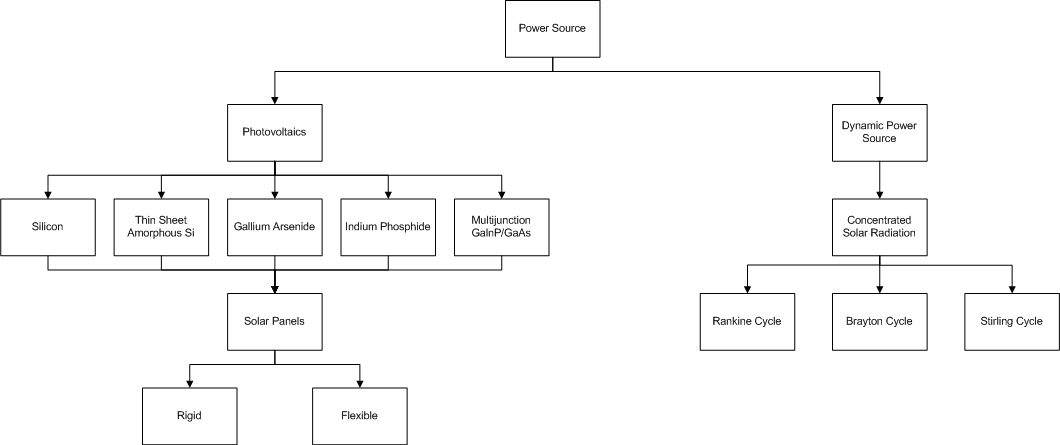
\includegraphics[width=\textheight, angle=90]{chapters/img/DOTeps_sourcePruned.png}
\caption{The pruned design option tree for the power source}
\label{fig:DOTeps_sourcePruned}
\end{figure}

\subsubsection{Power Storage}
\label{pruneEPS:Storage}
The only obvious candidate for power storage was secondary batteries because, as mentioned before, the lifetime of primary batteries is too short.
Of the most common secondary batteries, sodium-sulfur batteries are not an option for us because their operating temperature at 350 degrees Celsius is too high.

The pruned design option tree for the power source can be seen in figure \ref{fig:DOTeps_storagePruned}

\begin{figure}
\centering
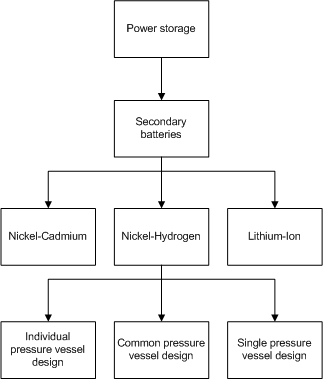
\includegraphics[width=0.35\textwidth]{chapters/img/DOTeps_storagePruned.png}
\caption{The pruned design option tree for the power storage}
\label{fig:DOTeps_storagePruned}
\end{figure}

\subsubsection{Power Distribution, Regulation and Control}
\label{pruneEPS:Distribution}
For the power distribution, regulation and control there were no obvious non-candidates. Because the power distribution, regulation and control depend on the type of power source, which depends on the payload power requirements, pruning will be done later on after these subsystems have been chosen --- this is done in the tradeoff.

The design option tree for the powersource can be seen in figure \ref{fig:DOTeps_reganddisPruned}

\begin{figure}
\centering
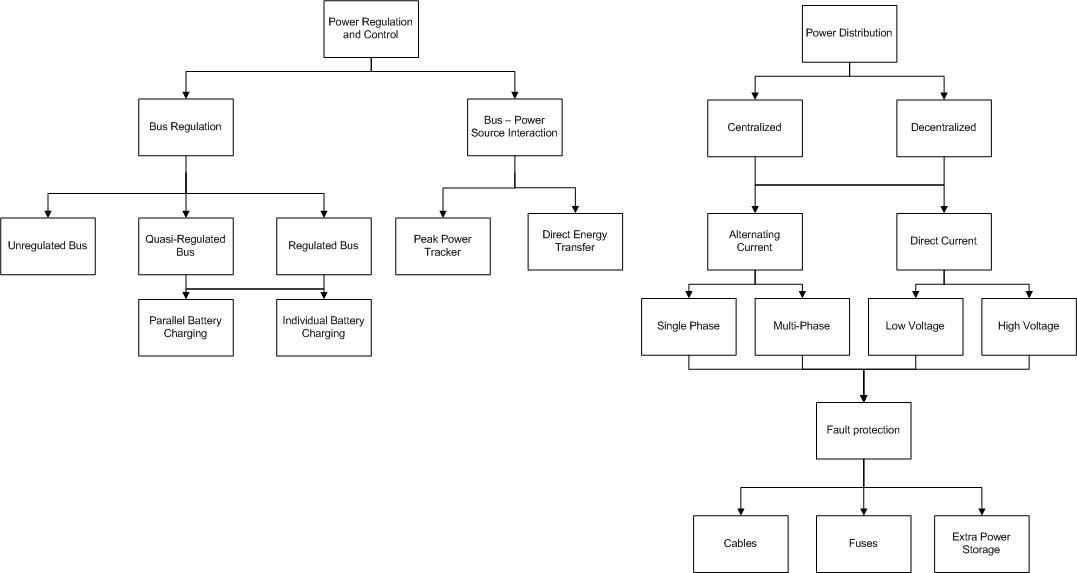
\includegraphics[width=\textheight, angle=90]{chapters/img/DOTeps_reganddisPruned.png}
\caption{The design option tree for the power distribution and regulation and control}
\label{fig:DOTeps_reganddisPruned}
\end{figure}

\subsection{Trade Method Rationale and Organization}
In this section the question of how the trade-off is done will be answered. First some additional information of the two options for the trade-off are given and afterwards the method and organization itself will be discussed.
After the pruning of the design option structure the only candidates left were photovoltaics and concentrated solar radiation together with an engine in a thermodynamic power cycle. 
After some further research the option of using concentrated solar radiation was also discarded. Almost no information was found about that
kind of powersource for use in space. Therefore it was decided to abandon this kind of power source because without any data or information 
it will not be possible to determine if that option is feasible. So that leaves only photovoltaics. 
Solar cells come in a lot of different types. The most common are crystalline solar cells, multijunction cells and thin film solar cells. Soon it was clear that crystalline would not be a good option. Multijunction cells have a higher efficiency while thin film cells have a lower mass and production cost. Because the efficiency, mass and production cost are the most important characteristics and crystalline solar cells do not excell in any of these areas (compared to multijunction and thin film cells), they will not be considered as an option for the power source.

\clearpage
\subsubsection{Multijunction Solar Cells}
A solar cell converts solar energy to electrical energy. When a photon hits the surface of a solar cell it is either reflected or transmitted.
If it is transmitted the energy it contains will excite an electron from the valence band to the conduction band. In the conduction band they have a higher energy than in the valence band, which allows them to move around. This happens in a so called pn-junction. Single crystalline solar cells have only one pn-junction whereas multijunction ones have more than one. Each pn-junction has a certain bandgap, depending on the material of the junction. The bandgap is the difference between the valence band and the conduction band.

This means that if a certain material has a bandgap of one electronvolt, one electronvolt of power needs to be given to an electron for it to be able to go from the valence band to the conduction band. From this it follows that one pn-junction will be able to use only part of the solar spectrum. Multijunction cells use several pn-junctions connected in series so that a larger part of the solar spectrum can be used.

Figure \ref{fig:multij_cell} gives a schematic representation of a triple-junction solar cell \cite{spectrolab}. The metallic contacts in aluminium are low resistivity electrodes that transfer the current from the solar panel to the power grid. They are present on the two sides of the structure but mainly on the backwards face so that the shadowing on the lit surface is reduced.

The anti-reflective coatings are primarily used to increase the transmission of the photons and correspondingly decrease the reflectance at the wavelengths that will be used.

Tunnel junctions provide a low electrical resistance and optically low-loss connection between two subcells. Without them, the p-doped region of the top cell would be directly connected with the n-doped region of the middle cell. Hence, a pn junction with opposite direction to the others would appear between the top cell and the middle cell. Consequently, the photovoltage will be lower. Tunnel junctions decrease this negative effect.

In figure \ref{fig:multij_cell}, the three materials for the pn-junctions that were used are Gallium-Indium-Diphosphor, Gallium-Arsenide and Germaniumn. These three pn-junctions cover a larger part of the solar spectrum than single junction solar cells, making them more efficient.

\begin{figure}[H]
\centering
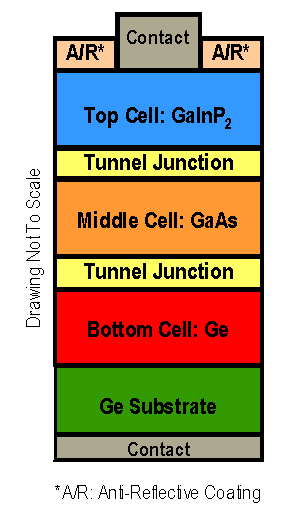
\includegraphics[height=0.4\textheight]{chapters/img/multijunction_solar_cell.png}
\caption{Schematic representation of a triple-junction solar cell}
\label{fig:multij_cell}
\end{figure}

Figure \ref{multi_irradiance} \cite{yastrebova} shows the range of wavelengths that eacht junction of a triple-junction cell absorbs. From this picture it is clear that multiple pn-junctions cover a far larger part of the solar spectrum than one single pn-junction.

\begin{figure}[H]
\centering
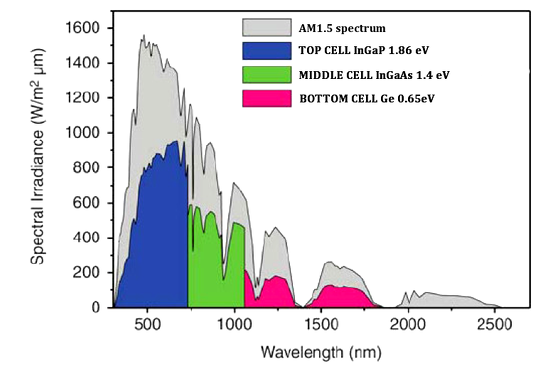
\includegraphics[height=0.4\textheight]{chapters/img/multijunction_spectral_irradiance.png}
\caption{Spectral irradiance of a triple-junction solar cell in function of the wavelength}
\label{multi_irradiance}
\end{figure}

\clearpage
\subsubsection{Thin Film Solar Cells}
Thin film solar cells are created by depositing one or more thin layers of photovoltaic material on a substrate. The thickness range of such a layer is wide and varies from a few nanometers to tens of micrometers. An example of a thin film solar cell shown in figure 
\ref{fig:thinfilm_cell}. Here the \ac{CIGS} cell is shown. Glass is commonly used as a substrate. A molybdenum layer is deposited which serves as the back contact and to reflect most unabsorbed light back into the absorber. The absorberlayer is a p-type layer. The most efficient absorber is a so called \ac{CIGS} absorber. It is a direct bandgap semiconductor with the highest absoprtance coefficient of all solar cells. \acl{CIGS} are the materials of the four thin layers of which it consists. A thin n-type buffer layer is added on top of the absorber. The buffer is overlaid with a thin, intrinsic Zinc-Oxide layer which is capped by a thicker, Aluminum doped Zinc-Oxide layer. Despite increasing the series resistance, the Zinc-Oxide layer is beneficial to cell performance. The Aluminum doped Zinc-Oxide serves as a transparent conducting oxide to collect and move electrons out of the cell while absorbing as little light as possible \cite{dhere}.

\begin{figure}
\centering
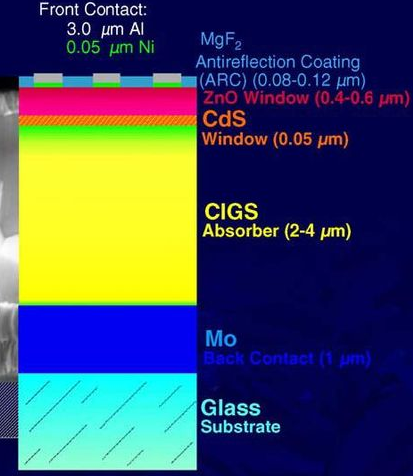
\includegraphics[width=0.4\textwidth]{chapters/img/thinfilm_solar_cell.png}
\caption{Schematic layout of a thin film CIGS solar cell}
\label{fig:thinfilm_cell}
\end{figure}

\clearpage
\subsubsection{Tradeoff Method and Rationale}
\label{TO_weight}
Now that the two candidates are known, the preparation of the trade-off can begin. Thin film \ac{CIGS} cells and triple-junction cells will be compared with each other with respect to certain criteria (i.e. cost, mass,...). For every criterium each candidate will receive points on a scale from one to ten, with ten being the highest. Each criterium will get a weight factor, depending on how important it is. To determine which solar cell type is the best, their points for each criterium will be multiplied with that criteriums weight factor. All these results will be added and the candidate with the highest total of points will be the best candidate for the mission. 
The first thing to do is to determine which criteria will be used. Efficiency, mass and cost are the three most important characteristics for the solar cells. They are also the ones that can deviate the most between different types of solar cells. Furthermore also the packing factor, degradation, solar cell height and resistance to vibrational noise during launch are trade-off criteria. 

The three most important characteristics, mass, cost and efficiency, are all given a weight factor of ten. The degradation of the cells is also an important criterium. A large degradation factor will increase the solar array area dramatically, especially for missions lasting a couple of years. Therefore its weight factor will be eight. The height of the cells influences the space each satellite needs when being launched. It could mean the difference of having an extra satellite per launcher, so it also is important. It received a 7 for its weight factor.

When considering a solar panel, not the whole panel is filled with solar cells. Part of is is taken up by wiring, the metal contacts of the cells, the loss in area because of the shape of the cells, \ldots All these factors are bundled in the packing factor. The higher the packing factor, the less solar array area is needed. It's weight is 7.

During take-off, the launcher and its payload experience large vibrational loads. The solar panels of the satellites need to be able to resist these loads. If they are affected too much by it some cells might be damaged, resulting in less power generation. The weight factor in this case is five. This is on the low side, because these vibrational loads will not be really destructive. 

\subsection{Tradeoff Summary}
In this section the summary of the trade-off process and the results will be discussed. For all the trade-off criteria, except for the resistance to vibrational loads, the marks each option receives are based on hard numbers. The candidate with the best characteristics will receive a ten and the other candidates marks are a fraction of that ten, based on the actual data. For example, if option 1 has a cost of 100 euros per watt, and option 2 costs 250 euros per watt, example 1 will receive a 10 for the criteia cost and example 2 will receive a four.

Table \ref{tab:TO_summary} lists the marks both candidates received and also their totals. From this it is obvious that the thin film \ac{CIGS} is the better candidate for our mission.

\begin{table}
\begin{tabular}{|c||c|c|c|}
\hline
 & Weight Factor & \multicolumn{2}{|c|}{Candidates} \\ \hline
 & & Thin film CIGS & Triple-junction \\ \hline
  \hline
 Efficiency & 10 & 4 & 10 \\ \hline
 Mass & 10 & 10 & 3 \\ \hline
 Cost & 10 & 10 & 4 \\ \hline
 Degradation & 8 & 10 & 9 \\ \hline
 Packing Factor & 7 & 8 & 8.5 \\ \hline
 Resistance to vibrational loads & 5 & 8 & 6 \\ \hline
 Cell Height & 7 & 10 & 2 \\ \hline
 \hline
 Total & & 486 & 345.5 \\ \hline
 \end{tabular}
 \caption{Trade-off table for the power source}
 \label{tab:TO_summary}
 \end{table}
 
The chosen thin film CIGS solar cells were developed by Dutch Space. They are some of the best avaiable and have been proven in flight with the Delfi-C3 satellite. For the triple-junction cells those developed by Azurspace were chosen. They are also on of the most efficient multijunction cells currently on the market and have been proven in flight. The data gathered for use of the exact numbers was taken from those two sources.

The efficiency of the CIGS cells is about $12\%$ and that of the triple-junction cells is $28\%$. This gives scores of ten and four respectively.
The mass of the cells are and $240g/m^2$ and $850g/m^2$, resulting in a ten and a three for the thin film CIGS and the multijunction respectively.
Degradation is low for both options, but the thin film CIGS has almost no open current and open voltage degradation, giving it a ten and the multijunction a nine. Average values of the packing factor found in the literature were used for the trade-off. The found values were $80\%$ and $85\%$, resulting in grades of eight and eight and a half. The height of the thin film CIGS cells is about $20\mu m$ giving it a ten. The triple-junction cells have a thickness of about $150\mu m$, giving it a two.
The grading of the resistance to vibrational loads was not done by comparing values because there are none available. It is known that stiffer panels have less resistance to vibrational loads than flexible panels, giving the thin film CIGS an advantage. This results in an eight for that type of cells and a six for the multijunction cells.

The data in the paragraph above was taken from \cite{esa_telecomm}, \cite{delfi_c3}, \cite{dutchspace}, \cite{spectrolab}, \cite{cubesatshop} and \cite{azurspace}.

For the power storage in the form of secondary batteries no real trade-off was needed. Nickel-Hydrogen batteries have been used extensively over the past years, but recently Lithium-Ion batteries have been tested for space application. Their specific energy can be up to three times as high as Nickel-Hydrogen batteries. It has been proven that, when kept within a certain temperature range, they have the same performance in space as on Earth \cite{LEO_li_ion}. This is why Lithium-Ion batteries are chosen for power storage.
\clearpage